\chapter{عملیات بیتی}

داده‌ها در برنامه‌های کامپیوتری به صورت بیت، یعنی اعداد ۰ و ۱ ذخیره می‌شوند.
این فصل به بررسی نمایش بیتی اعداد صحیح پرداخته و مثال‌هایی از نحوه کاربرد عملیات بیتی نشان می‌دهد.
عملیات بیتی در طراحی الگوریتم‌ها کاربردهای فراوانی دارد.

\section{نمایش بیتی}

\index{نمایش بیتی}

در برنامه‌نویسی، یک عدد صحیح $n$ بیتی در حافظه به صورت عدد دودویی شامل $n$ بیت ذخیره می‌شود.
به عنوان مثال، نوع \texttt{int} در C++ یک نوع ۳۲ بیتی است؛ یعنی هر عدد \texttt{int} از ۳۲ بیت تشکیل می‌شود.

نمایش بیتی عدد \texttt{int} با مقدار ۴۳:
\[00000000000000000000000000101011\]
اندیس‌گذاری بیت‌ها در این نمایش از راست به چپ انجام می‌شود.
جهت تبدیل نمایش بیتی $b_k \cdots b_2 b_1 b_0$ به یک عدد، از فرمول زیر استفاده می‌شود:
\[b_k 2^k + \ldots + b_2 2^2 + b_1 2^1 + b_0 2^0.\]
به عنوان مثال:
\[1 \cdot 2^5 + 1 \cdot 2^3 + 1 \cdot 2^1 + 1 \cdot 2^0 = 43.\]

نمایش بیتی اعداد می‌تواند \key{علامت‌دار} یا \key{بدون علامت} باشد.
معمولاً نمایش علامت‌دار استفاده می‌شود که در آن امکان نمایش هر دو نوع اعداد مثبت و منفی وجود دارد.
متغیر علامت‌دار $n$ بیتی می‌تواند مقادیر صحیح بین $-2^{n-1}$ تا $2^{n-1}-1$ را ذخیره کند.
به عنوان مثال، نوع \texttt{int} در C++ یک نوع علامت‌دار است، بنابراین متغیر \texttt{int} مقادیر صحیح بین $-2^{31}$ تا $2^{31}-1$ را در بر می‌گیرد.

اولین بیت در نمایش علامت‌دار، بیت علامت عدد است ($0$ برای اعداد نامنفی و $1$ برای اعداد منفی) و $n-1$ بیت باقی‌مانده بزرگی عدد را مشخص می‌کنند.
از روش \key{مکمل دو} استفاده می‌شود؛ در این روش عدد قرینه با معکوس کردن تمام بیت‌ها و سپس اضافه کردن یک واحد به عدد به دست می‌آید.

نمایش بیتی عدد \texttt{int} با مقدار $-43$:
\[11111111111111111111111111010101.\]

در نمایش بدون علامت، فقط اعداد نامنفی ذخیره می‌شوند، اما کران بالای مقادیر بزرگ‌تر است.
متغیر بدون علامت $n$ بیتی می‌تواند مقادیر صحیح بین $0$ تا $2^n-1$ را نگه دارد.
به عنوان مثال در C++، متغیر نوع \texttt{unsigned int} مقادیر بین $0$ تا $2^{32}-1$ را پوشش می‌دهد.

بین این دو نمایش رابطه ریاضی برقرار است:
عدد علامت‌دار $-x$ برابر با عدد بدون علامت $2^n-x$ است.
کد زیر نشان می‌دهد عدد علامت‌دار $x=-43$ برابر عدد بدون علامت $y=2^{32}-43$ است:
\begin{lstlisting}
int x = -43;
unsigned int y = x;
cout << x << "\n"; // -43
cout << y << "\n"; // 4294967253
\end{lstlisting}

اگر عددی از کران بالای نمایش بیتی فراتر رود، سرریز رخ می‌دهد.
در نمایش علامت‌دار، عدد بعد از $2^{n-1}-1$ برابر با $-2^{n-1}$ است و در نمایش بدون علامت، عدد بعد از $2^n-1$ برابر با $0$ خواهد بود.
کد زیر این رفتار را نشان می‌دهد:
\begin{lstlisting}
int x = 2147483647;
cout << x << "\n"; // 2147483647
x++;
cout << x << "\n"; // -2147483648
\end{lstlisting}

در ابتدا، مقدار $x$ برابر $2^{31}-1$ است.
این بزرگ‌ترین مقداری است که می‌توان در یک متغیر \texttt{int} ذخیره کرد،
بنابراین عدد بعدی پس از $2^{31}-1$ برابر $-2^{31}$ است.


\section{عملیات بیتی}

\newcommand\XOR{\mathbin{\char`\^}}

\subsubsection{عملگر And}

\index{and operation}

عملگر \key{and} یعنی $x$ \& $y$ عددی تولید می‌کند
که در جایگاه‌هایی دارای بیت یک است که هر دو عدد
$x$ و $y$ در آن جایگاه‌ها بیت یک داشته باشند.
به عنوان مثال، $22$ \& $26$ = 18، زیرا

\begin{center}
\begin{tabular}{rrr}
& 10110 & (22)\\
\& & 11010 & (26) \\
\hline
 = & 10010 & (18) \\
\end{tabular}
\end{center}

با استفاده از عملگر and می‌توان بررسی کرد که آیا عدد
$x$ زوج است یا خیر؛ چرا که اگر $x$ زوج باشد
$x$ \& $1$ = 0 و اگر $x$ فرد باشد
$x$ \& $1$ = 1 می‌شود.
به طور کلی‌تر، $x$ بر $2^k$ بخش‌پذیر است
دقیقاً زمانی که $x$ \& $(2^k-1)$ = 0 باشد.

\subsubsection{عملگر Or}

\index{or operation}

عملگر \key{or} یعنی $x$ | $y$ عددی تولید می‌کند
که در جایگاه‌هایی دارای بیت یک است که حداقل یکی
از مقادیر $x$ یا $y$ در آن جایگاه‌ها بیت یک داشته باشد.
به عنوان مثال، $22$ | $26$ = 30، زیرا

\begin{center}
\begin{tabular}{rrr}
& 10110 & (22)\\
| & 11010 & (26) \\
\hline
 = & 11110 & (30) \\
\end{tabular}
\end{center}

\subsubsection{عملگر Xor}

\index{xor operation}

عملگر \key{xor} یعنی $x$ $\XOR$ $y$ عددی تولید می‌کند
که در جایگاه‌هایی دارای بیت یک است که دقیقاً یکی
از مقادیر $x$ یا $y$ در آن جایگاه‌ها بیت یک داشته باشد.
به عنوان مثال، $22$ $\XOR$ $26$ = 12، زیرا

\begin{center}
\begin{tabular}{rrr}
& 10110 & (22)\\
$\XOR$ & 11010 & (26) \\
\hline
 = & 01100 & (12) \\
\end{tabular}
\end{center}

\subsubsection{عملگر Not}

\index{not operation}

عملگر \key{not} یعنی \textasciitilde$x$
عددی تولید می‌کند که تمام بیت‌های $x$
در آن معکوس شده‌اند.
رابطهٔ \textasciitilde$x = -x-1$ برقرار است،
به عنوان مثال، \textasciitilde$29 = -30$.

نتیجهٔ عملگر not در سطح بیت به طول نمایش بیتی بستگی دارد،
زیرا این عملیات تمام بیت‌ها را معکوس می‌کند.
به عنوان مثال، اگر اعداد ۳۲ بیتی از نوع
\texttt{int} باشند، نتیجه به شکل زیر است:

\begin{center}
\begin{tabular}{rrrr}
$x$ & = & 29 &   00000000000000000000000000011101 \\
\textasciitilde$x$ & = & $-30$ & 11111111111111111111111111100010 \\
\end{tabular}
\end{center}

\subsubsection{شیفت‌های بیتی}

\index{bit shift}

شیفت بیتی به چپ $x < < k$ تعداد $k$ بیت صفر
به انتهای عدد اضافه می‌کند،
و شیفت بیتی به راست $x > > k$
تعداد $k$ بیت انتهایی را از عدد حذف می‌کند.
به عنوان مثال، $14 < < 2 = 56$،
زیرا $14$ و $56$ متناظر با 1110 و 111000 هستند.
به همین ترتیب، $49 > > 3 = 6$،
زیرا $49$ و $6$ متناظر با 110001 و 110 هستند.

دقت کنید که $x < < k$
معادل ضرب $x$ در $2^k$ است،
و $x > > k$
معادل تقسیم $x$ بر $2^k$ و
گرد کردن آن رو به پایین به یک عدد صحیح است.

\subsubsection{کاربردها}

عددی به شکل $1 < < k$ دارای بیت یک در موقعیت $k$ است و تمام بیت‌های دیگر آن صفر هستند؛ بنابراین می‌توان از چنین اعدادی برای دسترسی به تک‌بیت‌های اعداد استفاده کرد.
به‌طور خاص، بیت $k$ام یک عدد یک است دقیقا زمانی که $x$ \& $(1 < < k)$ مخالف صفر باشد.
کد زیر نمایش بیتی یک عدد \texttt{int} به نام $x$ را چاپ می‌کند:

\begin{lstlisting}
for (int i = 31; i >= 0; i--) {
    if (x&(1<<i)) cout << "1";
    else cout << "0";
}
\end{lstlisting}

همچنین می‌توان با ایده‌های مشابه، تک‌بیت‌های اعداد را تغییر داد.
برای مثال، فرمول $x$ | $(1 < < k)$ بیت $k$ام $x$ را یک می‌کند،
فرمول $x$ \& \textasciitilde $(1 < < k)$ بیت $k$ام $x$ را صفر می‌کند،
و فرمول $x$ $\XOR$ $(1 < < k)$ بیت $k$ام $x$ را معکوس می‌کند.

فرمول $x$ \& $(x-1)$ آخرین بیت یک عدد $x$ را صفر می‌کند،
و فرمول $x$ \& $-x$ تمام بیت‌های یک را به جز آخرین بیت یک، صفر می‌کند.
فرمول $x$ | $(x-1)$ تمام بیت‌های پس از آخرین بیت یک را معکوس می‌کند.
همچنین دقت کنید که یک عدد مثبت $x$ توانی از دو است دقیقا زمانی که $x$ \& $(x-1) = 0$ باشد.

\subsubsection*{توابع اضافی}

کامپایلر g++ توابع زیر را برای شمارش بیت‌ها ارائه می‌دهد:

\begin{itemize}
\item
$\texttt{\_\_builtin\_clz}(x)$:
تعداد صفرها در ابتدای عدد
\item
$\texttt{\_\_builtin\_ctz}(x)$:
تعداد صفرها در انتهای عدد
\item
$\texttt{\_\_builtin\_popcount}(x)$:
تعداد یک‌ها در عدد
\item
$\texttt{\_\_builtin\_parity}(x)$:
زوج یا فرد بودن تعداد یک‌ها
\end{itemize}
\begin{samepage}

این توابع به صورت زیر قابل استفاده هستند:
\begin{lstlisting}
int x = 5328; // 00000000000000000001010011010000
cout << __builtin_clz(x) << "\n"; // 19
cout << __builtin_ctz(x) << "\n"; // 4
cout << __builtin_popcount(x) << "\n"; // 5
cout << __builtin_parity(x) << "\n"; // 1
\end{lstlisting}
\end{samepage}

اگرچه توابع بالا فقط از اعداد \texttt{int} پشتیبانی می‌کنند،
نسخه‌های \texttt{long long} این توابع نیز با پسوند \texttt{ll} در دسترس هستند.

\section{نمایش مجموعه‌ها}

هر زیرمجموعه از مجموعه $\{0,1,2,\ldots,n-1\}$ را می‌توان به عنوان یک عدد صحیح $n$ بیتی نمایش داد که بیت‌های یک آن مشخص می‌کنند کدام عناصر متعلق به زیرمجموعه هستند.
این یک روش کارآمد برای نمایش مجموعه‌ها است، زیرا هر عنصر تنها به یک بیت حافظه نیاز دارد و عملیات مجموعه را می‌توان به صورت عملیات بیتی پیاده‌سازی کرد.

برای مثال، از آنجا که \texttt{int} یک نوع داده ۳۲ بیتی است، یک عدد \texttt{int} می‌تواند هر زیرمجموعه‌ای از مجموعه $\{0,1,2,\ldots,31\}$ را نمایش دهد.
نمایش بیتی مجموعه $\{1,3,4,8\}$ برابر است با:
\[00000000000000000000000100011010,\]
که متناظر با عدد $2^8+2^4+2^3+2^1=282$ است.

\subsubsection{پیاده‌سازی مجموعه}

کد زیر متغیر \texttt{int} به نام $x$ تعریف می‌کند که می‌تواند زیرمجموعه‌ای از $\{0,1,2,\ldots,31\}$ نگه دارد.
سپس اعضای ۱، ۳، ۴ و ۸ را به مجموعه اضافه کرده و اندازه مجموعه را چاپ می‌کند.
\begin{lstlisting}
int x = 0;
x |= (1<<1);
x |= (1<<3);
x |= (1<<4);
x |= (1<<8);
cout << __builtin_popcount(x) << "\n"; // 4
\end{lstlisting}
سپس، کد زیر تمام اعضای متعلق به مجموعه را چاپ می‌کند:
\begin{lstlisting}
for (int i = 0; i < 32; i++) {
    if (x&(1<<i)) cout << i << " ";
}
// output: 1 3 4 8
\end{lstlisting}

\subsubsection{عمليات روی مجموعه‌ها}

عملیات روی مجموعه‌ها با عملگرهای بیتی پیاده‌سازی می‌شوند:

\begin{center}
\begin{tabular}{lll}
& نحو مجموعه‌ای & نحو بیتی \\
\hline
اشتراک & $a \cap b$ & $a$ \& $b$ \\
اجتماع & $a \cup b$ & $a$ | $b$ \\
متمم & $\bar a$ & \textasciitilde$a$ \\
تفاضل & $a \setminus b$ & $a$ \& (\textasciitilde$b$) \\
\end{tabular}
\end{center}

برای نمونه، کد زیر ابتدا مجموعه‌های $x=\{1,3,4,8\}$ و $y=\{3,6,8,9\}$ و سپس مجموعه $z = x \cup y = \{1,3,4,6,8,9\}$ را می‌سازد:

\begin{lstlisting}
int x = (1<<1)|(1<<3)|(1<<4)|(1<<8);
int y = (1<<3)|(1<<6)|(1<<8)|(1<<9);
int z = x|y;
cout << __builtin_popcount(z) << "\n"; // 6
\end{lstlisting}

\subsubsection{پیمایش زیرمجموعه‌ها}

کد زیر زیرمجموعه‌های $\{0,1,\ldots,n-1\}$ را پیمایش می‌کند:

\begin{lstlisting}
for (int b = 0; b < (1<<n); b++) {
    // process subset b
}
\end{lstlisting}
کد زیر زیرمجموعه‌های دقیقاً دارای $k$ عضو را پیمایش می‌کند:
\begin{lstlisting}
for (int b = 0; b < (1<<n); b++) {
    if (__builtin_popcount(b) == k) {
        // process subset b
    }
}
\end{lstlisting}
کد زیر زیرمجموعه‌های مجموعه $x$ را پیمایش می‌کند:
\begin{lstlisting}
int b = 0;
do {
    // process subset b
} while (b=(b-x)&x);
\end{lstlisting}

\section{بهینه‌سازی‌های بیتی}

بسیاری الگوریتم‌ها با عملیات بیتی بهینه می‌شوند.
این بهینه‌سازی‌ها پیچیدگی زمانی الگوریتم را تغییر نمی‌دهند، ولی بر زمان اجرای واقعی کد اثر زیاد دارند.
در این بخش مثال‌های این موضوع بررسی می‌شوند.

\subsubsection{فاصله همینگ}

\index{فاصله همینگ}
\key{فاصله همینگ} $\texttt{hamming}(a,b)$ بین دو رشته هم‌طول $a$ و $b$، تعداد جایگاه‌هایی است که دو رشته در آن اختلاف دارند.
برای نمونه:
\[\texttt{hamming}(01101,11001)=2.\]

مسئله: با داشتن فهرستی شامل $n$ رشته بیتی با طول $k$، کمینه فاصله همینگ بین دو رشته از فهرست محاسبه شود.
برای نمونه، پاسخ برای $[00111,01101,11110]$ برابر ۲ است، زیرا:
\begin{itemize}[noitemsep]
\item $\texttt{hamming}(00111,01101)=2$،
\item $\texttt{hamming}(00111,11110)=3$، و
\item $\texttt{hamming}(01101,11110)=3$.
\end{itemize}

یک روش سرراست برای حل مسئله،
بررسی تمام جفت‌های رشته‌ها و محاسبه
فاصله همینگ آن‌ها است
که الگوریتمی با زمان $O(n^2 k)$ به دست می‌دهد.
تابع زیر می‌تواند برای
محاسبه فاصله‌ها استفاده شود:
\begin{lstlisting}
int hamming(string a, string b) {
    int d = 0;
    for (int i = 0; i < k; i++) {
        if (a[i] != b[i]) d++;
    }
    return d;
}
\end{lstlisting}

با این حال، اگر $k$ کوچک باشد، می‌توان با ذخیره
رشته‌های بیتی به صورت اعداد صحیح و
محاسبه فواصل همینگ با استفاده از عملیات بیتی، کد را بهینه‌سازی کرد.
به‌ویژه اگر $k \le 32$ باشد، می‌توان رشته‌ها را صرفاً
به صورت مقادیر \texttt{int} ذخیره کرد و از
تابع زیر برای محاسبه فاصله‌ها بهره برد:
\begin{lstlisting}
int hamming(int a, int b) {
    return __builtin_popcount(a^b);
}
\end{lstlisting}
در تابع بالا، عملگر xor یک رشته بیتی می‌سازد
که در موقعیت‌هایی که $a$ و $b$ تفاوت دارند، بیت یک دارد.
سپس، تعداد بیت‌ها با استفاده از
تابع \texttt{\_\_builtin\_popcount} محاسبه می‌شود.

برای مقایسه پیاده‌سازی‌ها، فهرستی شامل ۱۰۰۰۰
رشته بیتی تصادفی به طول ۳۰ تولید شد.
با روش اول، جستجو ۱۳.۵ ثانیه طول کشید،
و پس از بهینه‌سازی بیتی،
فقط ۰.۵ ثانیه زمان برد.
بنابراین، کد بهینه‌شده با بیت تقریباً
۳۰ برابر سریع‌تر از کد اولیه بود.

\subsubsection{شمارش زیرشبکه‌ها}

به عنوان مثالی دیگر، مسئله زیر را در نظر بگیرید:
یک شبکه $n \times n$ داده شده است که
هر خانه آن سیاه (1) یا سفید (0) است.
تعداد زیرشبکه‌هایی را محاسبه کنید
که تمام گوشه‌های آن‌ها سیاه هستند.
برای نمونه، شبکه
\begin{center}
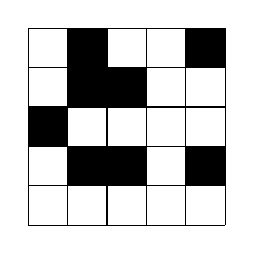
\begin{tikzpicture}[scale=0.5]
\fill[black] (1,1) rectangle (2,2);
\fill[black] (1,4) rectangle (2,5);
\fill[black] (4,1) rectangle (5,2);
\fill[black] (4,4) rectangle (5,5);
\fill[black] (1,3) rectangle (2,4);
\fill[black] (2,3) rectangle (3,4);
\fill[black] (2,1) rectangle (3,2);
\fill[black] (0,2) rectangle (1,3);
\draw (0,0) grid (5,5);
\end{tikzpicture}
\end{center}
شامل دو زیرشبکه از این نوع است:
\begin{center}
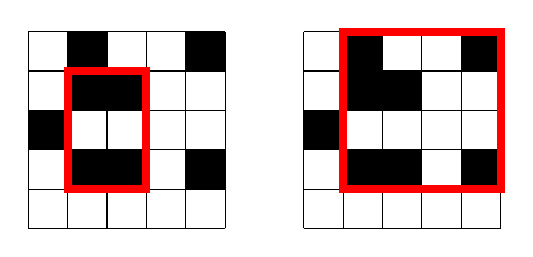
\begin{tikzpicture}[scale=0.5]
\fill[black] (1,1) rectangle (2,2);
\fill[black] (1,4) rectangle (2,5);
\fill[black] (4,1) rectangle (5,2);
\fill[black] (4,4) rectangle (5,5);
\fill[black] (1,3) rectangle (2,4);
\fill[black] (2,3) rectangle (3,4);
\fill[black] (2,1) rectangle (3,2);
\fill[black] (0,2) rectangle (1,3);
\draw (0,0) grid (5,5);

\fill[black] (7+1,1) rectangle (7+2,2);
\fill[black] (7+1,4) rectangle (7+2,5);
\fill[black] (7+4,1) rectangle (7+5,2);
\fill[black] (7+4,4) rectangle (7+5,5);
\fill[black] (7+1,3) rectangle (7+2,4);
\fill[black] (7+2,3) rectangle (7+3,4);
\fill[black] (7+2,1) rectangle (7+3,2);
\fill[black] (7+0,2) rectangle (7+1,3);
\draw (7+0,0) grid (7+5,5);

\draw[color=red,line width=1mm] (1,1) rectangle (3,4);
\draw[color=red,line width=1mm] (7+1,1) rectangle (7+5,5);
\end{tikzpicture}
\end{center}

الگوریتمی با زمان $O(n^3)$ برای حل مسئله وجود دارد:
تمام $O(n^2)$ جفت سطر را پیمایش کنید و برای هر جفت
$(a,b)$، تعداد ستون‌هایی را که در هر دو سطر دارای خانه سیاه
هستند در زمان $O(n)$ محاسبه کنید.
کد زیر فرض می‌کند که $\texttt{color}[y][x]$
نشان‌دهنده رنگ در سطر $y$ و ستون $x$ است:
\begin{lstlisting}
int count = 0;
for (int i = 0; i < n; i++) {
    if (color[a][i] == 1 && color[b][i] == 1) count++;
}
\end{lstlisting}
سپس، این ستون‌ها
شامل $\texttt{count}(\texttt{count}-1)/2$ زیرشبکه با گوشه‌های سیاه هستند،
زیرا می‌توان هر دو ستون از آن‌ها را برای تشکیل یک زیرشبکه انتخاب کرد.

برای بهینه‌سازی این الگوریتم، شبکه را به بلوک‌هایی
از ستون‌ها تقسیم می‌کنیم به طوری که هر بلوک شامل $N$
ستون متوالی باشد. سپس، هر سطر به صورت
فهرستی از اعداد $N$ بیتی ذخیره می‌شود که رنگ‌های
خانه‌ها را توصیف می‌کنند. اکنون می‌توانیم $N$ ستون را به طور همزمان
با استفاده از عملیات بیتی پردازش کنیم. در کد زیر،
$\texttt{color}[y][k]$ نشان‌دهنده
یک بلوک از $N$ رنگ به صورت بیت است.
\begin{lstlisting}
int count = 0;
for (int i = 0; i <= n/N; i++) {
    count += __builtin_popcount(color[a][i]&color[b][i]);
}
\end{lstlisting}
الگوریتم حاصل در زمان $O(n^3/N)$ کار می‌کند.

ما یک شبکه تصادفی به ابعاد $2500 \times 2500$ تولید کردیم
و پیاده‌سازی اولیه را با نسخه بهینه‌شده بیتی مقایسه نمودیم.
در حالی که کد اولیه $29.6$ ثانیه زمان برد،
نسخه بهینه‌شده با بیت با $N=32$ (اعداد \texttt{int}) تنها $3.1$ ثانیه
و با $N=64$ (اعداد \texttt{long long}) حدود $1.7$ ثانیه
زمان برد.

\section{برنامه‌نویسی پویا}

عملیات بیتی روشی کارآمد و مناسب برای
پیاده‌سازی الگوریتم‌های برنامه‌نویسی پویا ارائه می‌دهند
که وضعیت‌های آن‌ها شامل زیرمجموعه‌هایی از عناصر است،
زیرا چنین وضعیت‌هایی را می‌توان به صورت اعداد صحیح ذخیره کرد.
در ادامه به بررسی مثال‌هایی از ترکیب
عملیات بیتی و برنامه‌نویسی پویا می‌پردازیم.

\subsubsection{انتخاب بهینه}

به عنوان مثال اول، مسئله زیر را در نظر بگیرید:
قیمت‌های $k$ محصول در طول $n$ روز داده شده است
و می‌خواهیم هر محصول را دقیقاً یک بار بخریم.
با این حال، در هر روز مجاز به خرید حداکثر یک محصول هستیم.
حداقل قیمت کل چقدر است؟
به عنوان مثال، سناریوی زیر را در نظر بگیرید ($k=3$ و $n=8$):
\begin{center}
\begin{tikzpicture}[scale=.65]
    \draw (0, 0) grid (8,3);
    \node at (-2.5,2.5) {محصول 0};
    \node at (-2.5,1.5) {محصول 1};
    \node at (-2.5,0.5) {محصول 2};

    \foreach \x in {0,...,7}
        {\node at (\x+0.5,3.5) {\x};}
    \foreach \x/\v in {0/6,1/9,2/5,3/2,4/8,5/9,6/1,7/6}
        {\node at (\x+0.5,2.5) {\v};}
    \foreach \x/\v in {0/8,1/2,2/6,3/2,4/7,5/5,6/7,7/2}
        {\node at (\x+0.5,1.5) {\v};}
    \foreach \x/\v in {0/5,1/3,2/9,3/7,4/3,5/5,6/1,7/4}
        {\node at (\x+0.5,0.5) {\v};}
\end{tikzpicture}
\end{center}
در این سناریو، کمینه قیمت کل برابر $5$ است:
\begin{center}
\begin{tikzpicture}[scale=.65]
    \fill [color=lightgray] (1, 1) rectangle (2, 2);
    \fill [color=lightgray] (3, 2) rectangle (4, 3);
    \fill [color=lightgray] (6, 0) rectangle (7, 1);
    \draw (0, 0) grid (8,3);
    \node at (-2.5,2.5) {محصول 0};
    \node at (-2.5,1.5) {محصول 1};
    \node at (-2.5,0.5) {محصول 2};

    \foreach \x in {0,...,7}
        {\node at (\x+0.5,3.5) {\x};}
    \foreach \x/\v in {0/6,1/9,2/5,3/2,4/8,5/9,6/1,7/6}
        {\node at (\x+0.5,2.5) {\v};}
    \foreach \x/\v in {0/8,1/2,2/6,3/2,4/7,5/5,6/7,7/2}
        {\node at (\x+0.5,1.5) {\v};}
    \foreach \x/\v in {0/5,1/3,2/9,3/7,4/3,5/5,6/1,7/4}
        {\node at (\x+0.5,0.5) {\v};}
\end{tikzpicture}
\end{center}

فرض کنید $\texttt{price}[x][d]$ بیانگر قیمت محصول $x$
در روز $d$ باشد.
برای مثال، در سناریوی بالا $\texttt{price}[2][3] = 7$ است.
سپس، فرض کنید $\texttt{total}(S,d)$ کمینه قیمت کل
برای خرید زیرمجموعه $S$ از محصولات تا روز $d$ باشد.
با استفاده از این تابع، پاسخ مسئله
$\texttt{total}(\{0 \ldots k-1\},n-1)$ خواهد بود.

ابتدا، $\texttt{total}(\emptyset,d) = 0$،
زیرا خرید یک مجموعه تهی هزینه‌ای ندارد،
و $\texttt{total}(\{x\},0) = \texttt{price}[x][0]$،
زیرا برای خرید یک محصول در روز اول تنها یک راه وجود دارد.
سپس، رابطه بازگشتی زیر قابل استفاده است:
\begin{equation*}
\begin{split}
\texttt{total}(S,d) = \min( & \texttt{total}(S,d-1), \\
& \min_{x \in S} (\texttt{total}(S \setminus x,d-1)+\texttt{price}[x][d]))
\end{split}
\end{equation*}
این بدان معناست که یا در روز $d$ هیچ محصولی نمی‌خریم
یا محصول $x$ متعلق به $S$ را خریداری می‌کنیم.
در حالت دوم، $x$ را از $S$ حذف کرده و قیمت
$x$ را به قیمت کل اضافه می‌کنیم.

گام بعدی محاسبه مقادیر تابع با استفاده از برنامه‌نویسی پویا است.
برای ذخیره مقادیر تابع، آرایه‌ای تعریف می‌کنیم:
\begin{lstlisting}
int total[1<<K][N];
\end{lstlisting}
که در آن $K$ و $N$ ثابت‌های به اندازه کافی بزرگ هستند.
بعد اول آرایه متناظر با نمایش بیتی یک زیرمجموعه است.

ابتدا، حالت‌های $d=0$ این‌گونه پردازش می‌شوند:
\begin{lstlisting}
for (int x = 0; x < k; x++) {
    total[1<<x][0] = price[x][0];
}
\end{lstlisting}
سپس، رابطه بازگشتی به کد زیر تبدیل می‌شود:
\begin{lstlisting}
for (int d = 1; d < n; d++) {
    for (int s = 0; s < (1<<k); s++) {
        total[s][d] = total[s][d-1];
        for (int x = 0; x < k; x++) {
            if (s&(1<<x)) {
                total[s][d] = min(total[s][d],
                                    total[s^(1<<x)][d-1]+price[x][d]);
            }
        }
    }
}
\end{lstlisting}
پیچیدگی زمانی الگوریتم $O(n 2^k k)$ است.

\subsubsection{از جایگشت‌ها به زیرمجموعه‌ها}

با برنامه‌نویسی پویا، پیمایش روی جایگشت‌ها را اغلب می‌توان به پیمایش روی زیرمجموعه‌ها تبدیل کرد\footnote{این روش سال ۱۹۶۲ توسط ام. هلد (M. Held) و آر. ام. کارپ (R. M. Karp) معرفی شد \cite{hel62}.}.
علت:
تعداد جایگشت‌ها ($n!$) بسیار بزرگ‌تر از تعداد زیرمجموعه‌ها ($2^n$) است.
مثال: برای $n=20$ مقدار $n! \approx 2.4 \cdot 10^{18}$، اما $2^n \approx 10^6$.
بنابراین برای برخی مقادیر $n$، پیمایش زیرمجموعه‌ها کارا است اما پیمایش جایگشت‌ها غیرممکن است.

مثال:
آسانسوری با ظرفیت وزن $x$ وجود دارد.
$n$ نفر با وزن‌های مشخص می‌خواهند از همکف به بالاترین طبقه بروند.
حداقل تعداد دفعات حرکت آسانسور چقدر است اگر افراد با ترتیب بهینه سوار شوند؟

فرض کنید $x=10$ و $n=5$ و وزن‌ها چنین باشند:
\begin{center}
\begin{tabular}{ll}
شخص & وزن \\
\hline
0 & 2 \\
1 & 3 \\
2 & 3 \\
3 & 5 \\
4 & 6 \\
\end{tabular}
\end{center}
اینجا حداقل دفعات حرکت ۲ است.
یک ترتیب بهینه $\{0,2,3,1,4\}$ است
که افراد را به دو حرکت تفکیک می‌کند:
ابتدا $\{0,2,3\}$ (مجموع وزن ۱۰)،
سپس $\{1,4\}$ (مجموع وزن ۹).

مسئله با بررسی همه جایگشت‌های $n$ نفر در زمان $O(n! n)$ قابل حل است.
اما با برنامه‌نویسی پویا الگوریتمی در زمان $O(2^n n)$ به دست می‌آید.
ایده: برای هر زیرمجموعه از افراد دو مقدار محاسبه شود: حداقل دفعات حرکت لازم و حداقل وزن افراد در آخرین گروه.

فرض کنید $\texttt{weight}[p]$ وزن شخص $p$ باشد.
دو تابع تعریف می‌کنیم:
$\texttt{rides}(S)$ حداقل دفعات حرکت برای زیرمجموعه $S$،
و $\texttt{last}(S)$ حداقل وزن افراد در حرکت آخر.
برای نمونه در سناریوی بالا:
\[ \texttt{rides}(\{1,3,4\})=2 \hspace{10px} \textrm{و}
\hspace{10px} \texttt{last}(\{1,3,4\})=5,\]
زیرا حرکت‌های بهینه $\{1,4\}$ و $\{3\}$ هستند،
و حرکت دوم ۵ واحد وزن دارد.
هدف نهایی محاسبه $\texttt{rides}(\{0 \ldots n-1\})$ است.

می‌توانیم مقادیر تابع‌ها را به صورت بازگشتی محاسبه و سپس از برنامه‌نویسی پویا استفاده کنیم.
ایده کار، بررسی تمام افراد متعلق به $S$ و انتخاب بهینه آخرین فرد $p$ است که وارد آسانسور می‌شود.
هر انتخاب منجر به یک زیرمسئله برای زیرمجموعه کوچکتری از افراد می‌شود.
اگر $\texttt{last}(S \setminus p)+\texttt{weight}[p] \le x$ باشد،
می‌توانیم $p$ را به آخرین سفر اضافه کنیم.
در غیر این صورت، باید سفر جدیدی رزرو کنیم
که در ابتدا فقط شامل $p$ است.

برای پیاده‌سازی برنامه‌نویسی پویا،
آرایه‌ای تعریف می‌کنیم:
\begin{lstlisting}
pair<int,int> best[1<<N];
\end{lstlisting}
که برای هر زیرمجموعه $S$،
یک جفت $(\texttt{rides}(S),\texttt{last}(S))$ نگهداری می‌کند.
مقدار مربوط به گروه خالی را این‌گونه مقداردهی اولیه می‌کنیم:
\begin{lstlisting}
best[0] = {1,0};
\end{lstlisting}
سپس، آرایه را به این شکل پر می‌کنیم:

\begin{lstlisting}
for (int s = 1; s < (1<<n); s++) {
    // initial value: n+1 rides are needed
    best[s] = {n+1,0};
    for (int p = 0; p < n; p++) {
        if (s&(1<<p)) {
            auto option = best[s^(1<<p)];
            if (option.second+weight[p] <= x) {
                // add p to an existing ride
                option.second += weight[p];
            } else {
                // reserve a new ride for p
                option.first++;
                option.second = weight[p];
            }
            best[s] = min(best[s], option);
        }
    }
}
\end{lstlisting}
حلقه بالا تضمین می‌کند برای هر دو زیرمجموعه $S_1$ و $S_2$
که $S_1 \subset S_2$ باشد، زیرمجموعه $S_1$ قبل از $S_2$ پردازش می‌شود.
بنابراین، مقادیر برنامه‌نویسی پویا با ترتیب صحیح محاسبه می‌شوند.

\subsubsection{شمارش زیرمجموعه‌ها}

آخرین مسئله این فصل به شرح زیر است:
فرض کنید $X=\{0 \ldots n-1\}$ باشد و به هر زیرمجموعه $S \subset X$
یک عدد صحیح $\texttt{value}[S]$ نسبت داده شده باشد.
هدف ما محاسبه مقدار زیر برای هر $S$ است:
\[\texttt{sum}(S) = \sum_{A \subset S} \texttt{value}[A],\]
یعنی مجموع مقادیر زیرمجموعه‌های $S$.

به عنوان مثال، فرض کنید $n=3$ باشد و مقادیر به صورت زیر داده شده باشند:
\begin{multicols}{2}
\begin{itemize}
\item $\texttt{value}[\emptyset] = 3$
\item $\texttt{value}[\{0\}] = 1$
\item $\texttt{value}[\{1\}] = 4$
\item $\texttt{value}[\{0,1\}] = 5$
\item $\texttt{value}[\{2\}] = 5$
\item $\texttt{value}[\{0,2\}] = 1$
\item $\texttt{value}[\{1,2\}] = 3$
\item $\texttt{value}[\{0,1,2\}] = 3$
\end{itemize}
\end{multicols}
در این حالت، برای نمونه:
\begin{equation*}
\begin{split}
\texttt{sum}(\{0,2\}) &= \texttt{value}[\emptyset]+\texttt{value}[\{0\}]+\texttt{value}[\{2\}]+\texttt{value}[\{0,2\}] \\ 
                      &= 3 + 1 + 5 + 1 = 10.
\end{split}
\end{equation*}

به دلیل وجود $2^n$ زیرمجموعه،
یک راه‌حل ممکن بررسی تمام جفت‌های زیرمجموعه در زمان $O(2^{2n})$ است.
اما با برنامه‌نویسی پویا،
می‌توان مسئله را در زمان $O(2^n n)$ حل کرد.
ایده این است که روی مجموع‌هایی تمرکز کنیم که اعضای قابل حذف از $S$ در آن‌ها محدود شده‌اند.

فرض کنید $\texttt{partial}(S,k)$ برابر با مجموع مقادیر زیرمجموعه‌هایی از $S$ باشد، با این شرط که تنها عناصر $0 \ldots k$ اجازه دارند از $S$ حذف شوند.
برای مثال،
\[\texttt{partial}(\{0,2\},1)=\texttt{value}[\{2\}]+\texttt{value}[\{0,2\}],\]
زیرا تنها اجازه حذف عناصر $0 \ldots 1$ وجود دارد.
می‌توان مقادیر \texttt{sum} را با استفاده از مقادیر \texttt{partial} محاسبه کرد، زیرا
\[\texttt{sum}(S) = \texttt{partial}(S,n-1).\]
حالت‌های پایه برای این تابع عبارتند از
\[\texttt{partial}(S,-1)=\texttt{value}[S],\]
زیرا در این حالت هیچ عنصری نمی‌تواند از $S$ حذف شود.
سپس، در حالت کلی می‌توان از رابطه بازگشتی زیر استفاده کرد:
\begin{equation*}
    \texttt{partial}(S,k) = \begin{cases}
               \texttt{partial}(S,k-1) & k \notin S \\
               \texttt{partial}(S,k-1) + \texttt{partial}(S \setminus \{k\},k-1) & k \in S
           \end{cases}
\end{equation*}
در اینجا تمرکز روی عنصر $k$ است.
اگر $k \in S$ باشد، دو انتخاب وجود دارد: می‌توان $k$ را در $S$ نگه داشت یا آن را از $S$ حذف کرد.

روش بسیار هوشمندانه‌ای برای پیاده‌سازی محاسبه مجموع‌ها وجود دارد. می‌توان آرایه‌ای تعریف کرد:
\begin{lstlisting}
int sum[1<<N];
\end{lstlisting}
که مجموع هر زیرمجموعه را نگه‌داری خواهد کرد.
مقداردهی اولیه آرایه به شکل زیر انجام می‌شود:
\begin{lstlisting}
for (int s = 0; s < (1<<n); s++) {
    sum[s] = value[s];
}
\end{lstlisting}
سپس، می‌توان آرایه را به این صورت پر کرد:
\begin{lstlisting}
for (int k = 0; k < n; k++) {
    for (int s = 0; s < (1<<n); s++) {
        if (s&(1<<k)) sum[s] += sum[s^(1<<k)];
    }
}
\end{lstlisting}
این کد مقادیر $\texttt{partial}(S,k)$ را به ازای $k=0 \ldots n-1$ درون آرایه \texttt{sum} محاسبه می‌کند.
از آنجا که $\texttt{partial}(S,k)$ همواره بر پایه $\texttt{partial}(S,k-1)$ است، می‌توان از همان آرایه \texttt{sum} مجدداً استفاده کرد؛ امری که پیاده‌سازی بسیار کارآمدی را به دست می‌دهد.